\documentclass[12pt]{article}
\usepackage{float, amsmath, amssymb, amsthm, algorithm, algorithmic, graphicx, caption, subcaption, mathrsfs, color, cancel, verbatim, cite, authblk, mathtools}
\usepackage{enumitem}

\def\upint{\mathchoice%
    {\mkern13mu\overline{\vphantom{\intop}\mkern7mu}\mkern-20mu}%
    {\mkern7mu\overline{\vphantom{\intop}\mkern7mu}\mkern-14mu}%
    {\mkern7mu\overline{\vphantom{\intop}\mkern7mu}\mkern-14mu}%
    {\mkern7mu\overline{\vphantom{\intop}\mkern7mu}\mkern-14mu}%
  \int}
\def\lowint{\mkern3mu\underline{\vphantom{\intop}\mkern7mu}\mkern-10mu\int}

\let\oldemptyset\emptyset
\let\emptyset\varnothing

\setlength{\oddsidemargin}{0in}
\setlength{\evensidemargin}{\oddsidemargin}
\setlength{\textwidth}{6.5in}
\setlength{\topmargin}{-.25in}
\setlength{\headheight}{0in}
\setlength{\headsep}{0in}
\setlength{\topskip}{0in}
\setlength{\textheight}{9.5in}
\font\bigbf = cmbx10 scaled \magstep1
\font\medbf = cmbx10 scaled \magstephalf
\font\medrm = cmr10 scaled \magstephalf
\font\bigrm = cmr10 scaled \magstep1

\usepackage[english]{babel}
\usepackage[utf8]{inputenc}
\usepackage[colorinlistoftodos]{todonotes}

\title{Harmonic Analysis}
\begin{document}
\noindent \textbf{Lecture 3: Eyvindur Palsson} \\
\noindent www.math.vt.edu/people/palsson/pcmi.html \\

\noindent \textbf{Linear Algebra} \\
\noindent Let $V$ be a set of vectors of a field $F$. We define $f+g$, $\alpha f$, $f,g \in V$ and $\alpha \in F$.  \\

\noindent \textbf{Important Concepts to Recall}: Subspaces, linear operators, basis, ... \\

\noindent \textbf{Example}: Let $C[a,b] = \{f: [a,b]\rightarrow \mathbb{C} \mid f \text{ is continuous}\}$ be the space of continuous functions defined on the interval $[a,b]$. The space of continuous functions on $C[a,b]$ is a vector space. \\

\noindent \textbf{Complex Numbers} \\

\begin{figure}[H]
\centering
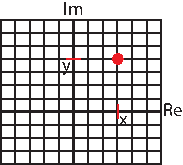
\includegraphics[width=0.25\textwidth]{ComplexNumberCoordinates.pdf}
\end{figure}


\noindent We denote the set of complex numbers with $\mathbb{C}$. A complex number contains the imaginary unit $i$, where $i^2=-1$. The modulus of a complex number $x+iy$ is defined as $\vert x + iy \vert =\sqrt{x^2+y^2}$. We can separate the imaginary and real parts of a complex number using $\text{Re}(x+iy)=x$ and $\text{Im}(x+iy)=y$. The conjugate of a complex number $\overline{x+iy} = x-iy$. Note that $(x+iy)\overline{(x+iy)} = \vert x+iy\vert^2$. Euler's formula $e^{i\theta} = \cos (\theta) + i \sin (\theta)$. 
(2) \\

\noindent From now on: Let $V$ be a vector space with scalars $\mathbb{K}=\mathbb{R}$ or $\mathbb{K} = \mathbb{C}$. \\

\noindent \textbf{Inner Product}: An inner product on a vector space $V$ over a field $\mathbb{K}$ is a function $\langle \cdot , \cdot \rangle: V \times V \rightarrow \mathbb{K}$ such that:

\begin{enumerate}[itemsep=0pt, parsep=0pt, partopsep=0pt, topsep=0pt]
\item For all $\textbf{v}_1 \textbf{v}_2 \in V$, $\langle \textbf{v}_1 , \textbf{v}_2 \rangle = \overline{\langle \textbf{v}_2 , \textbf{v}_1 \rangle}$.

\item For all $\textbf{v}_1, \textbf{v}_2, \textbf{v}_3 \in V$, $\langle \textbf{v}_1 + \textbf{v}_2 , \textbf{v}_3 \rangle = \langle \textbf{v}_1 , \textbf{v}_3 \rangle + \langle \textbf{v}_2 , \textbf{v}_3 \rangle$

\item For all $\textbf{v}_1, \textbf{v}_2 \in V$ and $\alpha \in \mathbb{K}$, $\langle \alpha \textbf{v}_1 , \textbf{v}_2 \rangle= \alpha \langle \textbf{v}_1 , \textbf{v}_2 \rangle$

\item For all $\textbf{v} \in V$, $\langle \textbf{v} , \textbf{v} \rangle \geq 0$ and $\langle \textbf{v} , \textbf{v} \rangle = 0$ if and only if $\textbf{u} = \textbf{0}$.  \\
\end{enumerate}

\noindent \textbf{Example}: Let $V= \mathbb{R}^d$, we define the inner product $\langle \cdot, \cdot \rangle$ with $\langle x, y \rangle = x\cdot y = x_1y_1 + \cdots + x_dy_d$. \\

\noindent \textbf{Example}: Let $V= \mathbb{C}^d$, we define the inner product $\langle \cdot, \cdot \rangle$ with $\langle x, y \rangle = x\cdot y = x_1\overline{y_1} + \cdots + x_d\overline{y_d}$. \\

\noindent \textbf{Example}: Let $V= C[a,b]$, we define the inner product $\langle \cdot, \cdot \rangle$ with $\langle f, g \rangle = \frac{1}{b-a} \int^b_a f(x)\overline{g(x)} dx$. \\

\noindent \textbf{Norm}: A norm on a vector space $V$ over a field $\mathbb{K}$ is a function $\Vert \cdot \Vert: V \rightarrow [0, \infty)$ such that:

\begin{enumerate}[itemsep=0pt, parsep=0pt, partopsep=0pt, topsep=0pt]
\item For all $\textbf{v}\in V$, $\Vert \textbf{v} \Vert \geq 0$ and $\Vert \textbf{v} \Vert = 0$ if and only if $\textbf{v}=\textbf{0}$.

\item For all $\textbf{v}\in V$ and $\alpha \in \mathbb{K}$, $\Vert \alpha \textbf{v} \Vert = \vert \alpha \vert \Vert \textbf{v} \Vert$.

\item For all $\textbf{v}_1,\textbf{v}_2 \in V$, $\Vert \textbf{v}_1 + \textbf{v}_2 \Vert \leq \Vert \textbf{v}_1 \Vert + \Vert \textbf{v}_2 \Vert$. \\
    \end{enumerate}

\noindent If $\langle \cdot , \cdot \rangle$ is an inner product on $V$, $\Vert \cdot \Vert$ is a norm on $V$ defined by $\Vert \textbf{v} \Vert= \sqrt{\langle \textbf{v}, \textbf{v} \rangle}$ for all $v \in V$. \\

\noindent The "norm" defined above is clear for the first two properties. The third requires the Cauchy-Schwartz inequality. \\

\noindent \textbf{Cauchy-Schwartz Inequality}: $\vert \langle f,g \rangle \vert \leq \Vert f \Vert \Vert g \Vert$. \\

\noindent To prove the third condition, consider the square of the problem statement,
\begin{align*}
\Vert f+g \Vert^2 &= \langle f+g, f+g \rangle \\
&= \vert f\Vert^2 + \langle f, g \rangle + \overline{\langle f,g \rangle} + \Vert g \Vert^2 \\
&\leq \Vert f \Vert^2 + 2 \Vert f \Vert \Vert g \Vert + \Vert g\Vert^2 \\
&= (\Vert f \Vert + \Vert g \Vert)^2
\end{align*}

\noindent \textbf{Example}: On $C[a,b]$ with 
$$\langle f, g \rangle = \frac{1}{b-a} \int^b_a f(x)\overline{g(x)} dx$$
we obtain
$$\Vert f \Vert_2 = \Big( \frac{1}{b-a} \int^b_a \vert f(x) \vert^2 dx \Big)^\frac{1}{2}$$
\noindent This is the $L_2$ norm. \\

\noindent \textbf{Orthogonality} \\
We say $f,g \in V$ are orthogonal if $\langle f, g \rangle = 0$. We say a set of vectors $\{\phi_1, \dots \phi_n\}$ are orthogonal if $\langle \phi_j, \phi_k \rangle$ whenever $j \not = k$ and $\phi_j \not= 0$ for all $j$.  \\

\noindent In addition, if $\Vert \phi_j \Vert = 1$ for all $j$, then $\{ \phi_1, \dots, \phi_n\}$ is orthonormal. \\

\textbf{Note}: Remember Gram-Schmidt. \\

\noindent \textbf{Pythagorean Theorem}: For orthogonal vectors $\textbf{v}_1, \dots, \textbf{v}_n$, $\Vert \textbf{v}_1 + \cdots + \textbf{v}_n \Vert^2 = \Vert \textbf{v}_1 \Vert^2 + \cdots + \Vert \textbf{v}_n \Vert^2$ \\

\noindent \textbf{Projections}
Let $\phi \in V$ with $\Vert \phi \Vert = 1$. The projection of $f$ in the direction of $\phi$ is 
$$\text{proj}_\phi(f):= \langle f,\phi \rangle \phi.$$

\noindent \textbf{Example}: Let $\overline{f} = (0,2)$ and let $\overline{\phi} = (\frac{1}{\sqrt{2}},\frac{1}{\sqrt{2}})$. Then,
$\text{proj}_{\overline{\phi}}(\overline{f}) = (1,1)$. (3) \\

\noindent \textbf{Definition}: Let $W_n$ be a subspace of $V$ with an orthonormal basis $\{\phi_1, \dots, \phi_n\}$. The projection of $f$ onto $W_n$ is 
$$\text{proj}_{W_n}(f):= \langle f, \phi_1\rangle \phi_1 + \cdots + \langle f, \phi_n \rangle \phi_n.$$

\noindent \textbf{Theorem}: 
$$\text{proj}_{W_n}(f)=f \text{ if and only if } f \in W_n$$
\noindent \textbf{Theorem}: \\
The vector $f-\text{proj}_{W_n}(f)$ is orthogonal to every vector in $W_n$. 



\end{document}